\begin{center}
    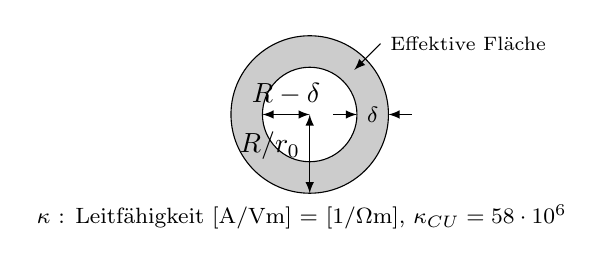
\begin{tikzpicture}
        %Kreise
        \draw[-,fill=black!20] (0,0) circle (1);              %äußerer Kreis
        \draw[-,fill=white] (0,0) circle (0.6);               %innerer Kreis

        %Pfeile
        \draw[latex-latex] (-0.6,0) -- (0,0) node[midway, above]{$R-\delta$};
        \draw[latex-latex] (0,-1) -- (0,0) node at (0,-0.4) [left]{$R/r_0$};

        \node at (0.8,0)[]{\footnotesize$\delta$};
        \draw[-latex] (0.3,0) -- (0.6,0);
        \draw[latex-] (1,0) -- (1.3,0);

        \draw[latex-] (0.566,0.566) -- (.9,.9) node[above, right]{\scriptsize{Effektive Fläche}};

        %Legende
        \node at (-0.1,-1.3)[]{\footnotesize{$\kappa$ : Leitfähigkeit [A/Vm] = [1/$\Omega$m], $\kappa_{CU} = 58 \cdot 10^6$}};
    \end{tikzpicture}
\end{center}
